\documentclass[twocolumn]{article}
\usepackage[utf8]{inputenc}
\usepackage[backend=biber]{biblatex}
\usepackage{graphicx} 
\usepackage{geometry}
\usepackage{amsmath}
\usepackage{booktabs}
\usepackage[T1]{fontenc}
\usepackage{babel}
\usepackage{cuted}
\usepackage{blindtext}
\usepackage{multicol}
\usepackage{adjustbox}
\usepackage[font=small,labelfont=bf]{caption}
 \geometry{
 a4paper,
 total={170mm,257mm},
 left=10mm,
 right=10mm,
 top=10mm}
\usepackage{lipsum} 

\makeatletter
\renewcommand{\paragraph}{\@startsection{paragraph}{4}{0ex}%
   {-3.25ex plus -1ex minus -0.2ex}%
   {1.5ex plus 0.2ex}%
   {\normalfont\normalsize\bfseries}}
\makeatother

\stepcounter{secnumdepth}
\stepcounter{tocdepth}

\title{\textbf{The More the Merrier}}
\author{
  Singh, Uttkarsh\\
  \texttt{uttkarsh.singh2004@gmail.com}
  \date{July 2021}}
  
\addbibresource{Reference-list.bib}

\renewenvironment{abstract}
 {\normalsize
  \begin{center}
  \bfseries \abstractname\vspace{-.5em}\vspace{0pt}
  \end{center}
  \list{}{
    \setlength{\leftmargin}{.5cm}%
    \setlength{\rightmargin}{\leftmargin}%
  }%
  \item\relax}
 {\endlist}
 
\begin{document}
\maketitle

\begin{abstract}
Due to the legislation of the Foundations for Evidence-Based Policy-making Act of 2018, publication papers are now required to be explicitly transparent with regard to the resources they utilize. Thus, a transparent and open approach was needed that would show how public data is being used in science and help the government make wiser and more transparent public investments. It would allow researchers and governments to upgrade from previously used tedious ad-hoc methods to an automated approach well founded by the modern techniques of Natural Language Processing and Transfer Learning. In this paper various baseline and intermediate approaches are explored that act as stepping stones to arrive at a final ensemble model consisting of Named Entity Recognition and Masked Language Modelling techniques from state-of-the-art NLP libraries namely SpaCy and BERT. Five models introduced in this paper bagged bronze medals in the Coleridge Initiative Featured Code Competition on Kaggle.
\end{abstract}
\textbf{Keywords} NER, Named entity recognition,
Dataset Extraction, Information Extraction, BERT, Dataset Mining, NLP,
Dataset Clustering, Doc2Vec, Dataset Search, dataset retrieval,
SpaCy, Masked Language Modelling.


\section{Introduction}
As a way of documenting and sharing results, the scholarly paradigm has relied extensively upon publication. As a result, scientific papers are typically the final word on a given scientific entity, such as how it was created, studied, and processed. But, unfortunately, this form of providing information has several flaws, the most prominent of which is that data and results are unreadable to systems due to their complex structuring. Additionally, close to 2.5 million articles [6] are said to be published each year and constantly growing [7]. And it is highly impractical for individual scholars to find crucial data in scientific publications. One might need to read hundreds of publications just to obtain a general understanding of the research in a certain field, and even then, there is no guarantee that they will not overlook crucial findings. \par

Crowd-sourcing is one approach for efficiently and cost-effectively doing manual, human-oriented jobs [8, 9, 10]. However, on the other hand, it is impractical due to the skill necessary to obtain scientific truths. The few current scientific databases and archives, such as the Japanese Polymer Data Handbook [11], are maintained by domain specialists and consequently expensive to maintain; as a result, they grow out of date quickly.\par

Owing to the fact that relying exclusively on humans to extract scientific facts from publications is impractical, automatic systems are required to deal with the rising velocity of publishing.Thus, the need for an efficient and transparent approach which would utilize natural language processing (NLP) to automate the discovery of how scientific data is referenced in publications is of vital importance.\par


\begin{center}
\hspace*{-0.8cm}
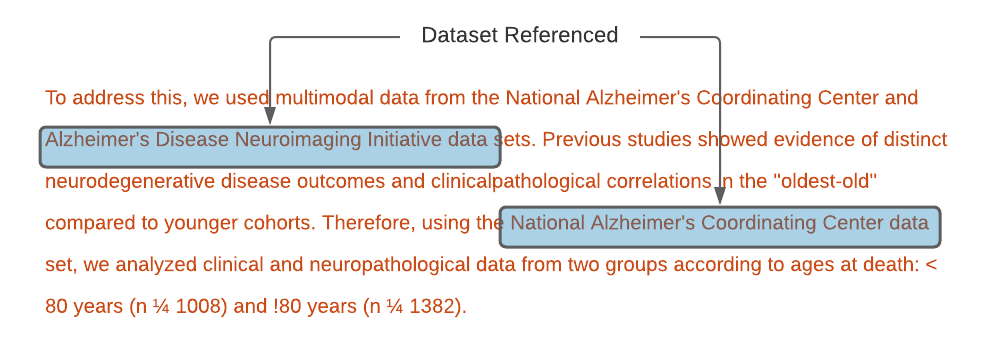
\includegraphics[scale=0.6]{Dataset Referenced.png}
\end{center}
\captionof{figure}{Visualisation of in-text dataset references}

As seen above, datasets and information centres are referenced all throughout research papers and the main objective of this paper is to explore several methods to extract these mentions automatically by utilizing the full text of scientific publications from numerous research areas. \par
	
Similar problems have been solved by researchers and NLP experts in the past- published in 2006, Fuchun Peng and Andrew McCallum presented a novel approach for constraint co-reference information extraction based on conditional random fields, however this approach focuses on the task of extracting various common fields from the headers and citation of research papers and ignore the various mentions that may be present in the raw text. \cite{peng-2006}. A conference paper, part of volume 337 of AISC proposed an approach towards information tracking in research papers using classification techniques \cite{priyanka-2015}. And a conference paper part of volume 381 of the same series presented a method of information extraction from research papers based on statistical approaches, in this paper SD Kavila and DF Rani use Key phrases and cue words to extract phrases of importance, similar to the rule-based approach discussed later in the paper. \cite{kavila-2015}. However, these methods and approaches only deem successful when applied on a relatively small amount of text and fail to generalize to a large corpus of data such as those found in publication papers. \par
	
In this paper, an aggregate ensemble network of state of the art NLP models namely BERT and SpaCy is proposed that uses Named Entity Recognition and Masked Language Modelling to achieve a generalized method of extracting the referenced datasets and is capable of achieving an accuracy score of 0.537 on a custom Kaggle competition dataset [12] that utilizes scientific publications from numerous research areas gathered from the CHORUS publisher members and other sources. In this paper, the final model is also compared to other baseline and intermediate models tested on the same dataset. \par
The dataset provided by Kaggle [12] comprises of 19,661 samples, but appears to have only 14,316 unique identifiers, implying that some publications contain more than one dataset. There are 45 different dataset titles as well as 130 different dataset classifications .\par

\section{Work done}
\subsection{SpaCy’s Rule-based Information Extraction}
SpaCy's pattern matcher and extractor was used to create a rudimentary baseline model. A set of rules were defined for the syntax and other grammatical properties of a natural language and these rules were then used to extract the necessary information from the text provided. \par

Information in text lies in the form of relations between different entities. We use this fact to extract structured information from unstructured data. After intensive exploratory data analysis the following examples of entity pairs were discovered.\par

\begin{center}
\hspace*{-0.1cm}
\includegraphics[scale=0.6]{Dataset Referenced Sentence Structure.png}\par
\end{center}
\captionof{figure}{Analysis of in-text word patterns}

Using this information, a Pattern Matcher for SpaCy was created using part-of-speech tags to extract pieces of the text that followed any of the variations of entity relations discovered. \par

\begin{center}
\hspace*{-0.4cm}
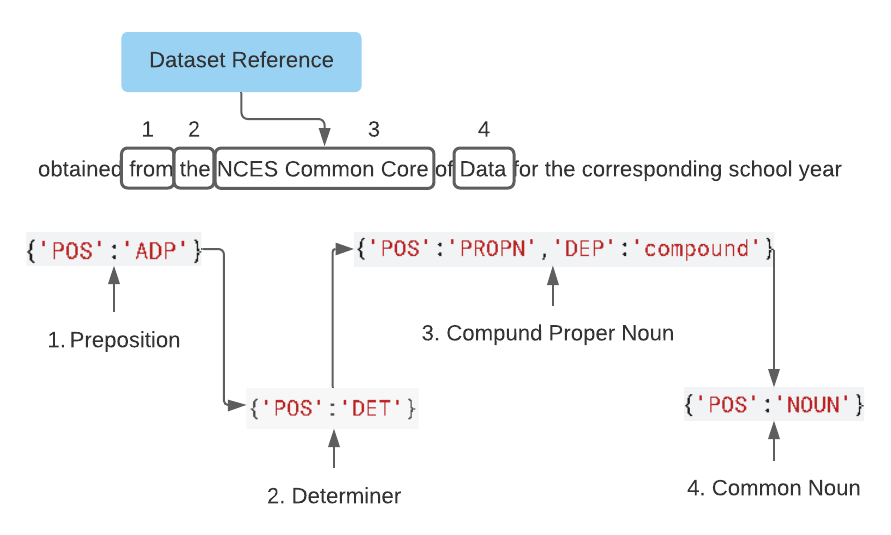
\includegraphics[scale=0.6]{Dataset Referenced Pattern Structure.png}
\end{center}
\captionof{figure}{Flow of SpaCy's custom built pattern matcher}

After analysing mentions of utilized datasets in research papers, the above generalized pattern was finalized. A preposition followed by a determiner followed by the proper noun dataset mention and finally a common noun depicting words like data, dataset, study, etc. SpaCy utilizes this grammar flow to extract phrases in text that match this pattern and then certain post-processing steps are required to extract the dataset mentions required.\par

Our Rule-Based model was able to achieve an accuracy score of 0.234 on the training dataset which is considered as the baseline accuracy for further explorations in this paper.\par

\subsection{Genism's Doc2Vec Classification}
Genism's Doc2Vec is a relatively modern approach to textual feature extraction, In contrast to traditional approaches to NLP such as one-hot encoding and bag-of-words models, the information about a word's meaning or context is captured as words and text are represented as multidimensional continuous floating point numbers. Doc2Vec is an NLP Tool for representing documents as a vector and generalization of the Word2Vec method. The goal of Doc2Vec is to create a numeric representation of a document, regardless of its length. Here, Mikilov and Le have used the word2vec model, and added another vector (Paragraph ID below)[13].\par
\begin{center}
\hspace*{-0.4cm}
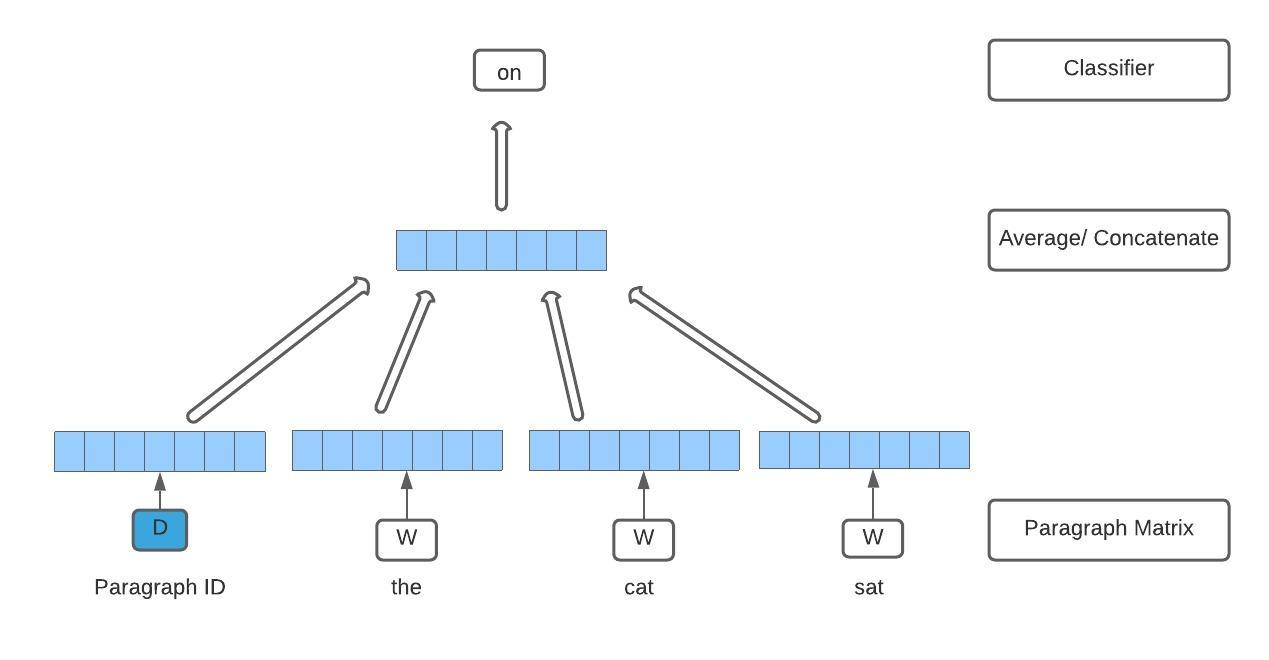
\includegraphics[scale=0.5]{Doc2Vec.jpeg}
\captionof{figure}{PV-DM Model}
\end{center}

The above sketch is a tiny addition to the CBOW model. Instead of merely utilising words to anticipate the following word, a document-unique feature vector is included. As a result, when the word vectors W are trained, the document vector D is also trained, and it carries a numeric representation of the document at the end of the training. \par 

This approach is known as the Distributed Memory Paragraph Vector model (PV-DM). It serves as a recollection, recalling what is absent from the current context — or as the paragraph's theme. The document vector seeks to represent the concept of a document, whereas the word vectors convey the concept of a word. \par 

Using the Doc2Vec algorithm the full text of research papers were converted to multidimensional vectors using the full-text corpus of words extracted and accumulated from the training dataset. These vectors were then used as "X-values" used to predict the "Y-values" or "labels" that happen to be the name(s) of the datasets utilized. This is where traditional machine learning makes an appearance.\par 

\begin{center}
\hspace*{-0.2cm}
\includegraphics[scale=0.4]{Doc2Vec.png}
\end{center}
\captionof{figure}{Flow of the Deep-Machine Learning approach}

A survey of multiple conventional machine learning algorithms was conducted and their respective accuracies on the training data compared. The probabilistic Random Forest model achieved the highest accuracy of 0.787 out of all the others and was used to match the generated vectors of the publication papers in the testing dataset to existing labels in the training set. The matched predictions were then string-matched in the document and the mentioning sentence extracted, forming the final predictions.\par

This deep-machine learning approach was able to outperform the baseline rule-based model by achieving an accuracy of 0.340 on the final testing set.
\subsection{Named Entity Recognition}
A bump in performance was observed from the rule-based approach when a blend of deep learning and machine learning algorithms were employed. Thus, a more sophisticated method needed to be applied. Named Entity Recognition is an advanced technique that fits the problem at hand. It utilizes deep learning and transfer learning techniques that can be implemented to extract trained labels (information extraction) from full-text documents such as research papers.\par

\subsubsection{SpaCy's Implementation}
SpaCy is an open-source software library for advanced natural language processing. It provides the fastest and most accurate syntactic analysis of any NLP library released to date. Another advantage of using spaCy is its custom-NER function, where the model can be trained to look for problem-specific entities instead of generic entities like "Person", "Location", "Organization", etc.\par

\begin{center}
\hspace*{-0.2cm}
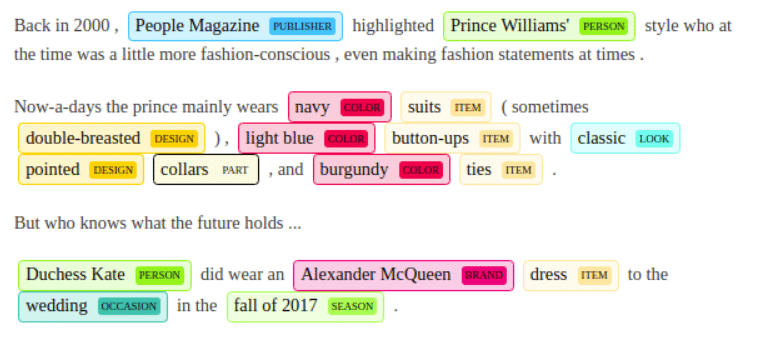
\includegraphics[scale=0.37]{SpaCy NER.png}
\end{center}
\captionof{figure}{Visual representation of spaCy's NER tagging [15]}

spaCy accepts training data as list of tuples where each tuple should contain the text and a dictionary. The dictionary should hold the start and end indices of the named entity in the text, and the category or label of the named entity. \\ For example,\\ \textbf{("analysing \emph{farm-level survey data} across the whole U.S.", {"entities": [(11, 32, "DATASET")]})}

The spaCy model functions like other deep learning architectures. \par

\begin{center}
\hspace*{-0.2cm}
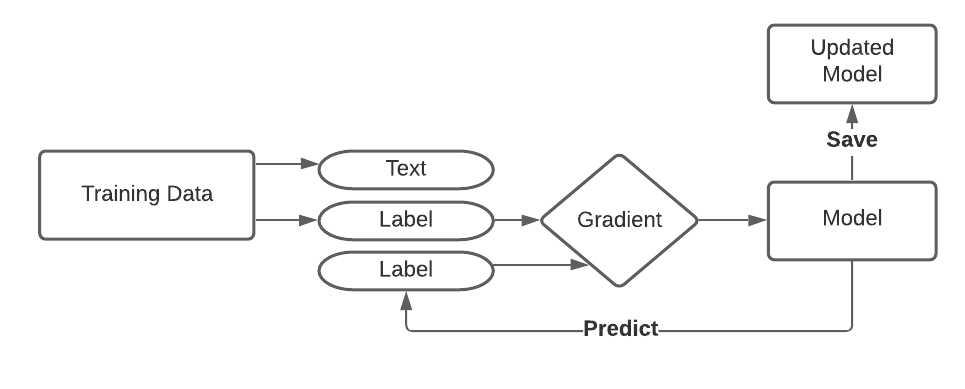
\includegraphics[scale=0.6]{SpaCy NER flow.png}
\end{center}
\captionof{figure}{SpaCy NER training flow}

Training data : Annotated data containing both text and their labels\\Text : Input text the model should predict a label for.\\Label : The label the model should predict.\\Gradient : Compare the prediction label with the actual label and adjusts its weights to improve the predictions. \\Save : Finally save the model\\The training data is usually passed in batches using the\\\textit{minibatch()} function of spaCy.\par

Although spaCy's implementation led to large improvements in accuracy, as it achieved a score of 0.433 on the testing set, it had a tendency to return null values for inputs with large uncertainties. This left space for improvement and a need to experiment with another advanced NLP library to fill the gaps.

\subsubsection{BERT Implementation}
\textbf{BERT} is a language representation model which represents \textbf{B}idirectional \textbf{E}ncoder \textbf{R}epresentations from \textbf{T}ransformers. [14] It pre-trains deep bidirectional representations from unlabeled text by jointly conditioning on both left and right context in all layers. Usually, the pre-trained BERT model is refined with just one or more output layers to provide state-of-the-art models for a wide range of specific tasks, including question answering and language inference, without requiring significant task-specific structural changes. \par

This section proposes the implementation of BERT for the task of extracting datasets from research papers using NER or Named Entity Recognition. \par 

The method \textbf{BertForTokenClassification} is used initially. Usually, in tasks like sequence classification, the entire sequence is classified to belong to 1 or 0 for binary classification and any 1 of the N classes for multi class classification. However, with Token Classification every single token(i.e words) in the sequence is classified as 1 of the N classes. \par 

\begin{center}
\hspace*{-0.2cm}
\includegraphics[scale=0.485]{BERT.jpeg}
\captionof{figure}{Token Classification in BERT}
\end{center}

Tokenization is simply the process of breaking down a sentence into words; however, Bert tokenizer only attempts to break down sentences that are already present in the vocabulary. If there are any complex words or terms that aren't in the vocabulary, Bert breaks them down into many sub-words, with each subword starting with "\#\#."

\begin{center}
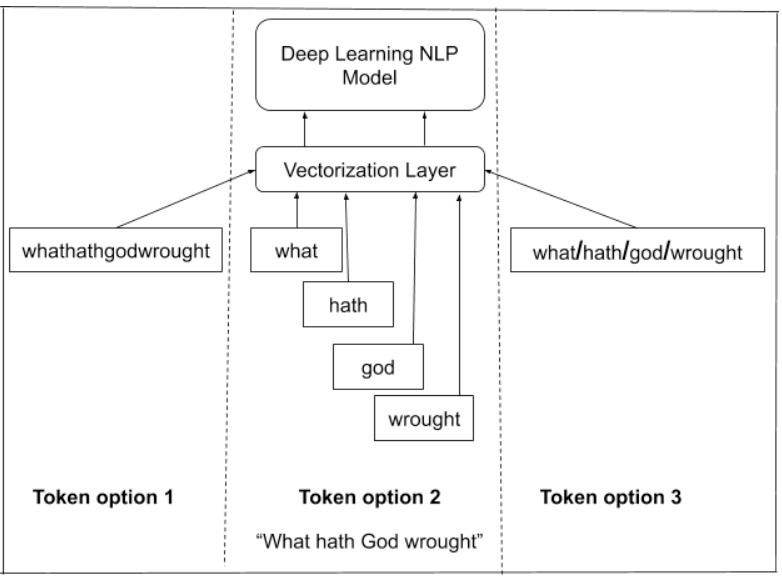
\includegraphics[scale=0.3]{tokenizer.jpeg} 
\captionof{figure}{Working of Word Tokenization} 
\end{center}

The function form\_labels() is utilized where the labelled data is fed to the algorithms. Consider the following sentence for example: 

"control samples were selected from individuals who had participated in genomewide association studies performed by our group 787 samples from the neurogenetics collection at the coriell cell repository and 728 from the baltimore longitudinal study of aging blsa" \par

\textbf{Label:} \textit{"genomewide association studies", "baltimore longitudinal study of aging"}. \par

\textbf{Portion to label:} \textit{"control samples were selected from individuals who had participated in \textbf{genomewide association studies} performed by our group 787 samples from the neurogenetics collection at the coriell cell repository and 728 from the \textbf{baltimore longitudinal study of aging blsa"}} \par 

Tokenizing the sentence as: \par
\textit{['control', 'samples', 'were', 'selected', 'from', 'individuals', 'who', 'had', 'participated', 'in', 'genome', '\#\#wide', 'association', 'studies', 'performed', 'by', 'our', 'group', '78', '\#\#7', 'samples', 'from', 'the', 'ne', '\#\#uro', '\#\#gen', '\#\#etic', '\#\#s', 'collection', 'at', 'the', 'co', '\#\#rie', '\#\#ll', 'cell', 'repository', 'and', '72', '\#\#8', 'from', 'the', 'baltimore', 'longitudinal', 'study', 'of', 'aging', 'b', '\#\#ls', '\#\#a']} \par 

Followed by label tokenization: \par 
\textit{[['genome', '\#\#wide', 'association', 'studies'], ['baltimore', 'longitudinal', 'study', 'of', 'aging']]} \par 

For each tokenized label, the tokenized train sentence is looped, and when a match is found, they are labelled as 'B' (Beginning) and 'I' (Inside) while the rest of them as 'O' (other). Since there are two labels the train sentence is looped twice. At the end of the 1st loop for ['genome', '\#\#wide', 'association', 'studies'], the label looked like this: \par 

\textit{['O', 'O', 'O', 'O', 'O', 'O', 'O', 'O', 'O', 'O', 'B', 'B', 'B', 'B', 'O', 'O', 'O', 'O', 'O', 'O', 'O', 'O', 'O', 'O', 'O', 'O', 'O', 'O', 'O', 'O', 'O', 'O', 'O', 'O', 'O', 'O', 'O', 'O', 'O', 'O', 'O', 'O', 'O', 'O', 'O', 'O', 'O', 'O', 'O']} \par 

At the end of the 2nd loops for ['baltimore', 'longitudinal', 'study', 'of', 'aging'] the final label looked like this: \par 

\textit{['O', 'O', 'O', 'O', 'O', 'O', 'O', 'O', 'O', 'O', 'B', 'B', 'B', 'B', 'O', 'O', 'O', 'O', 'O', 'O', 'O', 'O', 'O', 'O', 'O', 'O', 'O', 'O', 'O', 'O', 'O', 'O', 'O', 'O', 'O', 'O', 'O', 'O', 'O', 'O', 'O', 'B', 'B', 'B', 'B', 'B', 'O', 'O', 'O']} \par 

Once all the train datasets are passed to the model, the input sentence returned a dictionary of ids. The ids contains array-encoded numbers that can then be decoded to reveal the index position of the labelled tokens in the Bert vocabulary. \par 

BERT is known to outperform initial SpaCy models by an impressive percentage. For the domain-specific task of data identification and extraction, in this paper, BERT's fine tuned large-uncased model surpassed its predecessor and achieved a score of 0.531 on the test set.

\subsection{Masked Language Modelling}
A Transformers based deep learning model capable of bidirectionality outperformed previous models and left space for an approach that is utilized in BERT's pre-training phase alongside Next Sentence Prediction. 

Masked language modelling is an example of auto-encoding language modelling where an output needs to be reconstructed from a intentionally corrupted input. We mask one or more words in a fixed-length sentence and have the model predict those masked elements based on the context of words on both sides of the mask. By training BERT with such an objective, the model can essentially learn the statistical properties of word sequences.

\begin{center}
\hspace*{-0.55cm}
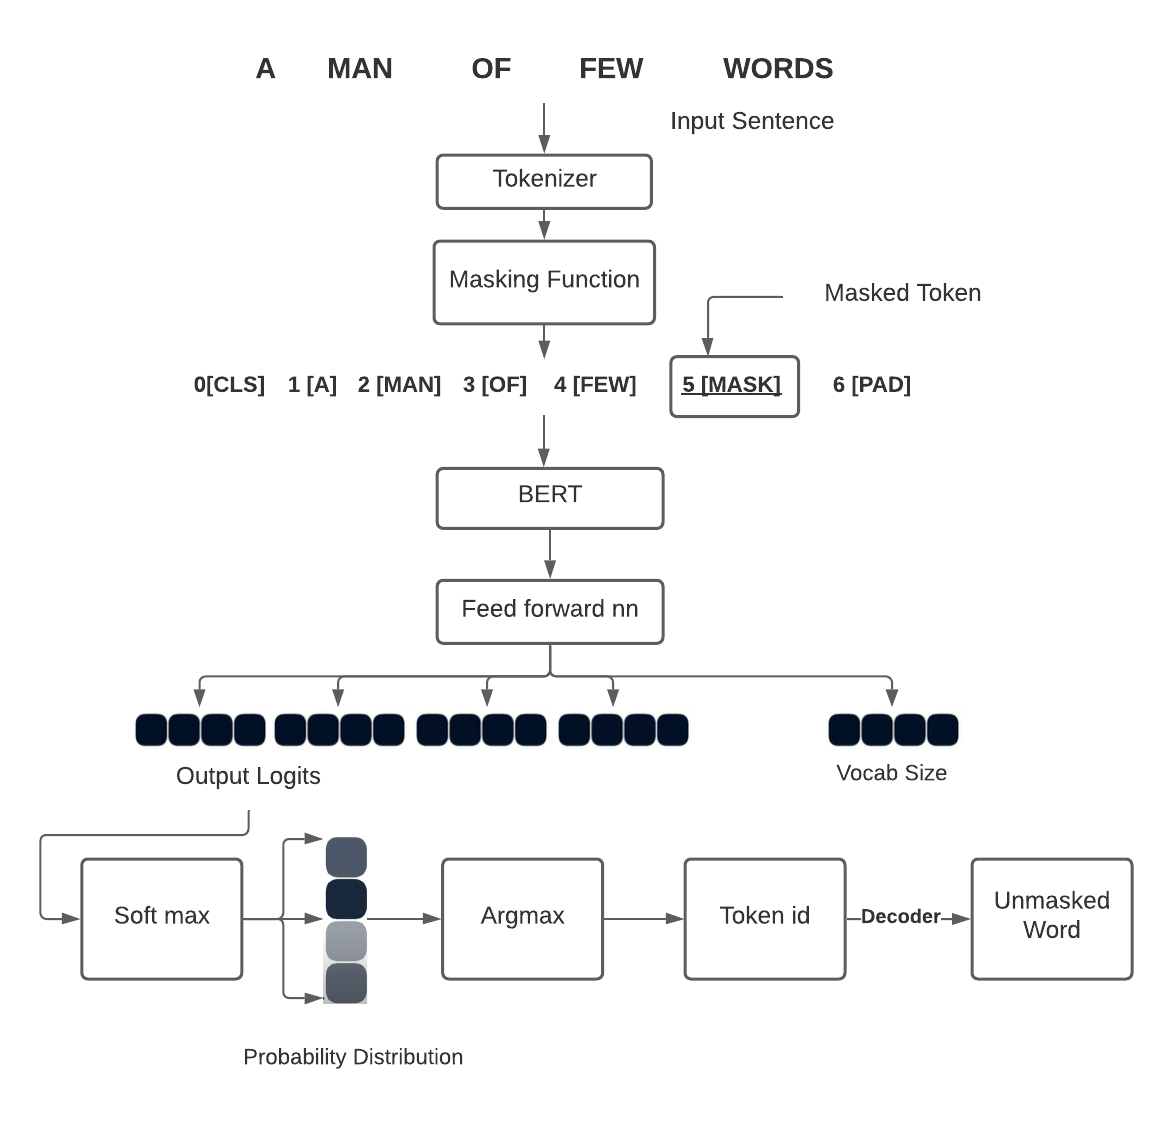
\includegraphics[scale=0.24]{MLM.png} 
\captionof{figure}{Low-level overview of Masked Language Modelling} 
\end{center}

A overview of the workings of BERT's MLM training phase is depicted above. Generally BERT masks approximately 15\% of the input sentence tokens [14]. 

We propose Masked Dataset Modelling with BERT's large-cased model. For the downstream task of dataset extraction certain "sentence candidates" were chosen. After observation during EDA it was found that most of the dataset names consisted of only words with an upper-cased-first-letter and some stopwords like on, in, and, etc. (e.g. Early Childhood Longitudinal Study, Trends in International Mathematics and Science Study). From 19,661 unprocessed full-text research papers, sentences with recurring upper-cased first letter words (not bound by grammar rules) were chosen as candidates for Masked Language Modelling.

Thus, a simple approach was formulated:
\begin{itemize} 
\item Locate and extract every sequence of capitalized words (may include stopwords).
\item Replace each sequence with one of 2 special symbols \$ or \#, implying if that sequence represents a dataset name(\$) or not(\#).
\item Have BERT learn the MLM task and fine-tune. 
\end{itemize}

Thus, from each paper in the training set hundreds of "positive" and "negative" candidates were extracted. Positive candidates were sentences that contained the [DATASET SYMBOL] while negative candidates were those the contained the [NON-DATASET SYMBOL].

The training data for BERT MLM now consisted of 57993 positive + 183485 negative samples.

After collating the data and fine-tuning the 'bert-large-cased' model the model achieved an accuracy score of 0.571, further surpassing its preceding Named Entity Recognition model and SpaCy's Implementation of the same.

\subsection{Conglomerated Ensemble Model}
Ensemble techniques are a type of machine learning methodology that integrates numerous base models to create a single best-fit predictive model. It helps improve machine learning results by combining several models. This approach allows the production of better predictive performance compared to a single model. \par 

This technique combines several machine learning techniques into one predictive model in order to decrease variance (bagging), bias (boosting), or improve predictions (stacking). Bagging which stands for bootstrap aggregation is one way to reduce the variance of an estimate is to average together multiple estimates. \par 

The need for an ensemble technique was felt because out of the survey of models a few performed well on certain subsets of the data while produced null predictions for other subsets. At the same time other state of the art models performed well on those subsets. Thus an aggregate model of previously implemented models was created which utilized BERT's Named Entity Recognition and Masked Language Modelling as well as SpaCy's NER. \par 

The models that were aggregated in this Ensemble technique filled in the gaps left by other models and allowed for more consistent and accurate predictions leading to an outperforming accuracy score of 0.581 on the public test set.

\begin{center}
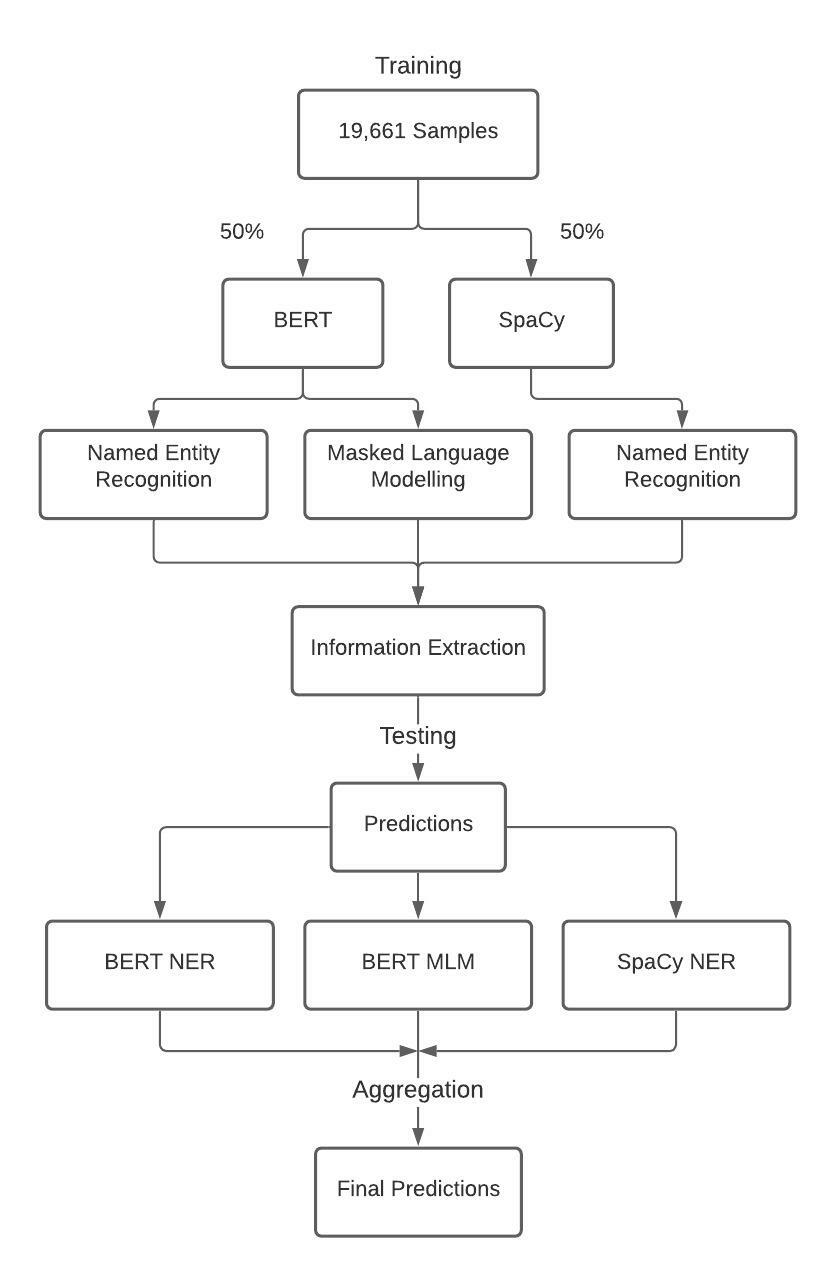
\includegraphics[scale=0.6]{ensemble.jpeg}
\captionof{figure}{An Over-view of the Ensemble approach}
\end{center}

\begin{table*}[ht]
	\centering
	\begin{tabular}[t]{lcc}\\
		\toprule
		Model&Approach&Similarity Score\\
		\midrule
		SpaCy's Rule Based Matching&Machine Learning&0.234\\
		Genism's Doc2Vec&Deep Machine Learning&0.340\\
		SpaCy's NER&Deep Learning&0.433\\
		BERT NER&Transfer Learning&0.531\\
		BERT MLM&Transfer Learning&0.571\\
		Conglomerate Ensemble&Aggregation&0.581\\
		\bottomrule
	\end{tabular}
\caption{Table of results}
\end{table*}%

\section{Results \& Discussion}
Our findings hint that the task of information extraction from unlabelled full-text research papers is a job not well suited for rudimentary and rule-based models as seen from the low accuracy score achieved by spaCy's Matcher, this may have branched from the variations and complexity of languages. An upward improvement was seen as the complexity of the architecture and the approach increased. A higher score was gained by time-heavy and resource-heavy models like BERT's large pre-trained models. It is clear that it is an inefficient task to identify elements from text based on grammar rules alone. Simple classification approaches also produce only mediocre results. 

The task of extracting datasets used specifically from research papers is quite peculiar and the most similar approaches to our methods have been used to extract the meta-data (Journal, Year, Title, Author, etc.) from these papers in different languages. F Peng and Andrew McCallum used Conditional Random fields [2] to achieve an overall accuracy of 98.3% and an average F1 score of 93.9 through all the fields. For this similar task multiple papers have used three widely used datasets namely CORA, FLUX-CiM and UMASS that were developed in 1999–2000, 2007 and 2013 respectively. As reflected in a survey [16] done by Zara Nasar, Syed Waqar Jaffry and Muhammad Kamran Malik, Conditional Random Fields were able to produce state-of-the-art results on all three datasets with an average score of 0.9648 through all the fields. Andrew McCallum and Wei Li used CRFs in conjunction with Named Entity Recognition [17] to achieve an overall testing score of 84.04 in the English language and 68.11 when the model was tested on German, their models were tested on lexicons built automatically from HTML data scraped from the Web. 

Thus, even for a relatively unexplored area such as dataset extraction Conditional Random Fields holds promise, especially when used in aggregation with other non-statistical methods.

However, during intermediate exploration, it was discovered that a rule based method could be used to fill in the gaps left by the state of the art models utilized in this model. Due to the complexity and robustness of theses modern implementations of deep and transfer learning, like BERT, spaCy and Doc2Vec they occasionally fail to output any prediction at all, for example most labels produced by the fine-tuned large-cased model needed to be "filtered" which led to losing the low confidence predictions, however, in most real world applications, a 45\% confidence prediction does better than a null outcome.

This technique of sharing training data and aggregating outputs has proven useful in other fields such as in the extraction of medical information from clinical texts [18]. Youngjun Kim and Stéphane M Meystre trained 4 sequential classifiers and created a stacked ensemble consisting of these concept extraction models trained on the shared training data. Their end-to-end system was able to achieve an overall micro-averaged recall, precision, and F1 score of 92.52\%, 81.88\% and 86.88\%, respectively. Their study demonstrated that a stacked ensemble with a search-based structured prediction algorithm achieved a better performance by effectively integrating the output of individual classifiers.

Similar to Youngjun Kim and Stéphane M Meystre's contibution, in the 2013 paper by Madian Khabsa and C. Lee Giles their framework incorporates an ensemble of multiple information extractors to obtain high accuracy on the BioCreative CHEMDNER Task.

However, achieving similarity scores these high with these methods can prove to be a very tedious task and sometimes unfeasible when it comes to dataset extraction. The data used in the BioCreative Chemdner task as well as medical information extraction, is more processed than not and contains identifiers that simplify the localization of the data to be extracted. For example, in a prescription given by a clinic the names of medicines and their respective doses could be placed under specified columns making it easier to unsheathe. On the other side of the fence, dataset extraction from full length research papers that are sometimes larger than 40 pages, is a context driven task, dataset names may be mentioned in the abstract and conclusion or detected a hundred times over throughout the text or not mentioned at all, dataset names may also be changed, altered or written in short form as seen multiple times in the data this paper utilizes.

In conclusion, this paper suggests that multiple models working in congregation will often outperform individual standalone models even when applied to dataset extraction from full-length research papers, as justified by the results achieved.


\begin{thebibliography}{12}
\bibitem{SD Kavila and DF Rani}
SD Kavila and DF Rani. “Information Extraction from Research Papers Based on Statistical Methods. In: Advances in Intelligent Systems and Computing (2015), pp. 573–580. doi: 10 . 1007 /978-81-322-2526-3\_59.

\bibitem{F Peng and A McCallum}
F Peng and A McCallum. “Information extraction from research papers using conditional random fields”. In: Information Processing \& Management 42.4 (2006), pp. 963–979. doi: 10.1016/j.ipm.2005.09.002.

\bibitem{JSVSH Priyanka et al}
JSVSH Priyanka et al. “Information Tracking from Research Papers Using Classification Techniques”. In: Advances in Intelligent Systems and Computing (2015), pp. 153–160. doi: 10 . 1007 /978-3-319-13728-5\_17.

\bibitem{HH Yang}
HH Yang. “Hierarchical Classification Methods of Chinese Scientific Papers Based on Extracting Key Words”. In: Applied Mechanics and Materials 40 (2010), pp. 1006–1011. doi: 10.4028/www.scientific.net/amm.40-41.1006.

\bibitem{K Adnan and R Akbar}
K Adnan and R Akbar.“An analytical study of information extraction from unstructured and multidimensional big data”. In: Journal of Big Data 6.1 (2019). doi: 10.1186/s40537-019-0254-8.

\bibitem{Ware, M., Mabe, M.}
Ware, M., Mabe, M.: The STM report: an overview of scientific and scholarly journal publishing. Technical report, International Association of Scientific, Technical and Medical Publishers (2015)

\bibitem{Fortunato, S., et al}
Fortunato, S., et al.: Science of science. Science 359(6379) (2018).  https://doi.org/10.1126/science.aao0185, https://science.sciencemag.org/content/359/6379/eaao0185

\bibitem{Bonney, R., et al}
Bonney, R., et al.: Citizen science: a developing tool for expanding science knowledge and scientific literacy. Bioscience 59(11), 977–984 (2009)

\bibitem{Bonney, R., et al}
Bonney, R., et al.: Next steps for citizen science. Science 343(6178), 1436–1437 (2014)

\bibitem{Cohn, J.P}
Cohn, J.P.: Citizen science: can volunteers do real research? Bioscience 58(3), 192–197 (2008)

\bibitem{Ohama, Y}
Ohama, Y.: Handbook of Polymer-Modified Concrete and Mortars: Properties and Process Technology. William Andrew, Norwich (1995)

\bibitem{Kaggle}
Kaggle. Competition: coleridgeinitiative-show-us-the-data.

\bibitem{Quoc V. Le, Tomas Mikolov}
le2014distributed, Distributed Representations of Sentences and Documents, Quoc V. Le and Tomas Mikolov, 2014.

\bibitem{Jacob Devlin and Ming-Wei Chang and Kenton Lee and Kristina Toutanova}
BERT: Pre-training of Deep Bidirectional Transformers for Language Understanding,Jacob Devlin and Ming-Wei Chang and Kenton Lee and Kristina Toutanova, 2019.

\bibitem(N. Sharma)
Sharma, N. (2019, November 30). How to create custom NER in Spacy – ConfusedCoders. Confused Coders. https://confusedcoders.com/data-science/deep-learning/how-to-create-custom-ner-in-spacy

\bibitem{Zara Nasar, Syed Waqar Jaffry, Muhammad Kamran Malik}
Nasar, Z., Jaffry, S.W. \& Malik, M.K. Information extraction from scientific articles: a survey. Scientometrics 117, 1931–1990 (2018). https://doi.org/10.1007/s11192-018-2921-5

\bibitem{Andrew McCallum, Wei Li.}
Andrew McCallum and Wei Li. 2003. Early results for named entity recognition with conditional random fields, feature induction and web-enhanced lexicons. In Proceedings of the seventh conference on Natural language learning at HLT-NAACL 2003 - Volume 4 (CONLL '03). Association for Computational Linguistics, USA, 188–191. DOI:https://doi.org/10.3115/1119176.1119206

\bibitem{Youngjun Kim, Stéphane M Meystre}
Kim, Youngjun, and Stéphane M Meystre. “Ensemble method-based extraction of medication and related information from clinical texts.” Journal of the American Medical Informatics Association : JAMIA vol. 27,1 (2020): 31-38. doi:10.1093/jamia/ocz100

\bibitem{Madian Khabsa, C. Lee Giles}
Khabsa, Madian and C. Lee Giles. “An Ensemble Information Extraction Approach to the BioCreative CHEMDNER Task.” (2013).
\end{thebibliography}
\end{document}

